\documentclass[12pt]{article}
\usepackage{fullpage}
\usepackage{multirow}
\usepackage{graphicx}

%NOTE: This proposal is intended as 
% (1) A template for your document
% (2) An example of the writing.
% It is not intended as an example of the project's scope:
% The project proposed in this sample is purposefully WAY
% beyond the scope of the class.

\begin{document}
\begin{center}
% Project Title
    {\Large A Qt5-based Music Player} 

\vspace*{20pt}
% List your group members' names and NetIds
\begin{tabular}{lc}
Allen Yin& asy13 \\
Jieqing Dai & jd260 \\
\end{tabular}
\end{center}
%Give a brief (one paragraph) summary of the project.

For our project, we will develop a functionally lightweight music player with a GUI based on the Qt5 framework. This music player will have all the basic functionalties of a media player, in addition to playlist support.


\section{Functional Requirements}
% Describe the functional requirements.
% This is what you would need to do for a mid-B to a low-A
% Be *as specific as possible here*.  If you specifically 
% want to make clear that certain functionality is outside
% the scope of what you propose, please be sure to do so.


\begin{description}
    \item[Playback] We will use either Qt5's built-in MediaPlayer widget or a different media playback library to handle the decoding of the media files and the system calls to the playback devices. The type of media files will be limited to mp3 files in the basic implementation. The essential functionalities, which also translate to individual GUI elements, include:
        \begin{itemize}
            \item Play/Pause button to start or pause the playback of the current media file.
            \item A slider that shows the progress of the playback, which can be manually dragged to advance/rewind the song. When the music player is in focus, the left/right arrowkeys can be used instead of manually dragging the slider to advance/rewind the song by 3 seconds.
            \item Next/Back buttons to skip to the next or previous song in the current playlist. If the current playlist has only 1 song, nothing happens. If it's currently playing the first song of the playlist, \emph{Back} plays the last song of the playlist; if the last song of the playlist is playing, \emph{Next} plays the first song.
        \end{itemize}
    \item[Playlist] The \emph{Playlist} is a collection of media files that we are currently playing, and is shown via the \emph{Playlist} area. The user can add songs to the playlist via dragging selection from the \emph{Library/File Browser} area and dropping into the \emph{Playlist} area. The \emph{Playlist} area will have columns to display the song's Name, Artist, and Album information, based on the mp3 file's metadata. These information can be modified within this area. A search box will be available for querying the playlist. There will also be  checkboxes/buttons for different playlist options including shuffle, repeat, and loop. Playlists can be saved for future use.
    \item[Library/File Browser] The \emph{Library} area allows the user to navigate the filesystem to add folders/files to his collection. Once a folder/file is selected, the mp3 files contained will be processed for the metadata and added to the area. The Library will display the songs in artist items, which when expanded will show the individual song names. A search box will be available to query through the collection. The data for the Library will be stored via Sqlite, for which Qt5 provides support. The \emph{Library} will also contain a list of known/saved playlists.
    \item[Title Area] The \emph{Title Area} shows the Name, Artist, and Album of the current song being played, as well as the volumn control.
    \item[GUI] The GUI will be implemented in Qt5 for its cross-platform support. Ubuntu 14.04 is our default platform. A mockup of the application is shown below.
\end{description}

\begin{figure}[h]
    \centering
    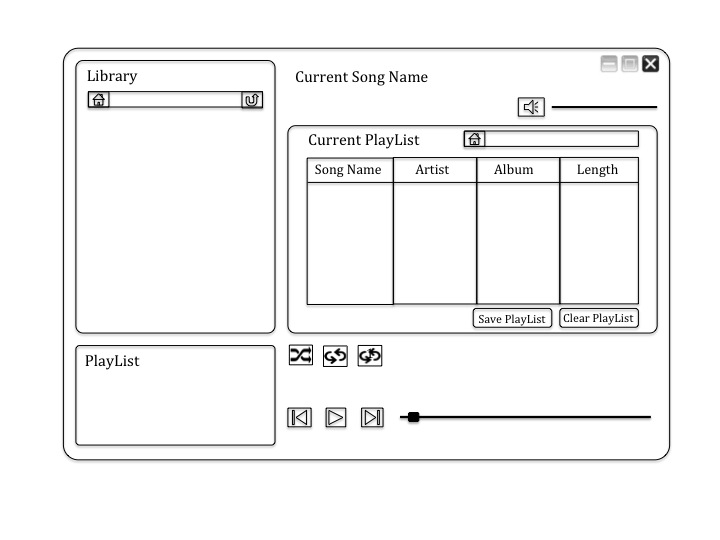
\includegraphics[width=0.9\textwidth]{mockup.jpg}
    \caption{Mock-up of our Music Player's GUI}
\end{figure}

\section{Stretch Goals}
% Once you have fulfilled your basic requirements, what do you
% see as the more ambitious steps to take you into the high-A range?
% Its good if you can be precise, but, for these it is acceptable
% to be a bit more vague.

\begin{description}
    \item[Platform Support] Our first stretch goal will be to provide support of the application on both Linux and MacOSX, and maybe Windows (as the file structure and playback devices organization is different from Unix systems).
    \item[Media Support] Our second stretch goal will be to provide support to media formats other than mp3, such as m4a, wav, wma.
    \item[Lyrics Fetching] Our third stretch goal will be to provide for lyrics fetching. The lyrics for the song current playing will be fetched through select sites from the internet and the \emph{Playlist} area will be resized dynamically to display lyrics.
    \item[System Tray] Our last stretch goal is to allow the application to sit in the OS' application tray when the 'x' button is clicked, rather than closing and exiting. In this state, a notification box with the new song's information will pop up whenever the current song is changed.
\end{description}


\section{Software Design Plan}
% In this section, you should lay out a rough plan to build your 
% software.  How do you split the work amongst a team?  What
% pieces are you going to build first?  Can you test along the way?
% Are there any other things you need to build which are not
% part of your ``deliverables''? (e.g., to help test)
% What is your project timeline?  How many person-hours of work
% do you expect for each task?
%
% The key thing here is that I want to see that you have thought
% about what it will take to accomplish your goal, and planned
% on a reasonably sized project
%
% I should feel like you have a plan to at least get through your
% functional requirements within the timeline of this project
% (and picking a project substanative enough for a final project).
%
% A good rule of thumb is about 30 hours per person, since
% you no longer have  videos to watch and this project spans 3.5 weeks

Our first step will be to familiarize ourselves with Qt, and to create the core media playback section of our application (as described in the \emph{Playback} section of our functional description and GUI mockup). This first iteratioin will allow us to load one song at a time for playback. This will be split between two people as it is the most important core functionality.

After the development of the core playback, one of us will work on the \emph{Library} area while the other on the \emph{Playlist} area. The Library person will need to integrate Sqlite with our application. We will then work on integrating the two functionalities together, enabling drag and drop between the two areas and saving Playlists.

Then we will finalize our GUI design - adding in the Title Area and tweaking the look and feel. Af this stage, we will focus on testing and optimizing for resource usage. Once we are satisfied with the basic application, we will work down the list of our stretch goals.

\begin{table}
\begin{center}
\begin{tabular}{|c|c|c|c|c|c|c|}
\hline
\multirow{2}{*}{Task}      &  \multicolumn{3}{|c|}{Expected Person-Hours}    &  \multirow{2}{*}{Start} & \multirow{2}{*}{End} & \multirow{2}{*}{Person} \\
                           &  Implement     & Test       & Debug            &                         &                      &                         \\
\hline
\hline
  Media Playback&   6            & 2          & 1                & Nov 3                   & Nov 6                & Allen, Jieqing  \\
  Library               &   6            & 2          & 1                & Nov 6                   & Nov 12               & Allen \\
  Playlist             &   6            & 2          & 1                & Nov 6                   & Nov 12               & Jieqing \\
  Integration   & 10 & 4 & 3 & Nov 12 & Nov 17 & Allen, Jieqing\\
\hline
 \multicolumn{7}{|c|}{Stretch Goals} \\
\hline
MacOS Support &   4           & 1         &   3                & Nov 17                  & Nov 20               & Jieqing\\
Media Support &   3           & 2         &   3                & Nov 17                  & Nov 20               & Allen \\
Lyrics Fetching &   6           & 2         &   2                & Nov 20                  & Nov 25               & Allen, Jieqing \\
System Tray &   4           & 3         &   3                & Nov 25                  & Nov 27               & Allen, Jieqing \\

\hline
\end{tabular}
\caption{Summary of work breakdown and time expectations.}
\label{Table:planSummary}
\end{center}
\end{table}

Table~\ref{Table:planSummary} sumarizes our expected time breakdown by task, as well as who is planning to do each task, and what our exected schedule of starting/completing the tasks is.


\section{Specific Expertise}
% Lay out the specific technical expertise (beyond just programming)
% that your group needs to succeed.  If you have that expertise
% already or if you have/know of the resources you need, point that
% out.  If you lack information and will need me to help you find it,
% this is the time to let me know.
% 
% That last part is important, so I'll say it again:
% If there is specific technical expertise that you might lack,
% tell me NOW.  If you propose (complex artificial intelligence thing
% I know nothing about), don't know to me a week before the deadline
% and tell me that you don't know anything about AI...

This project requires a proficient knowledge with the Qt framework, especially its support for Multimedia and Sqlite. None of us have used it, however, Qt has a strong community and we should be able to find help online.

We are familiar with both Linux and MacOSX, so platform support should not be too difficult. Since Qt is platform independent, we will also be able to find help online.
\end{document}
